\begin{frame}
	\frametitle{Bayesian linear mixed effects models}
	
	\begin{itemize}
		\item Easier model fit: complex models converge \textit{by definition}
		\item Answer the question we care about: what's the support for the hypothesis given the data? 
		\item Intuitive interpretation: frequentist estimates are often interpret in a Bayesian manner \cite{nicenboim2016statistical}
		\item Support for the hypothesis is not quantified by the implausibility of the null.

	\end{itemize}

\only<2>{
	\begin{minipage}{.6\textwidth}
			Is $p$ the probability that the null is true?\\ What are we doing with $p=0.06$?
	\end{minipage}
	\hfill
	\begin{minipage}{.35\textwidth}
	\begin{figure}
		\centering
		
\includegraphics[scale =.15]{gfx/p.jpg}
	\end{figure}
\end{minipage}
}
\end{frame}


\begin{frame}
	\frametitle{Bayesian linear mixed effects models}
	
	\begin{itemize}
		\item Bayesian inference based on the \textbf{Posterior} distribution approximated from the product of the \textbf{Likelihood} and the \textbf{Prior}:

		\begin{itemize}
		\item[(a)] Plausible values for model parameters -- \textbf{Prior}.
		\item[(b)] Probability model of the data generating process -- \textbf{Likelihood}.

	\end{itemize}
		\item Sophisticated sampling techniques: Monte Carlo Markov Chain
		
		\item Sampling is used to approximate the posterior distribution by creating probability distributions of plausible parameter values.
	\end{itemize}
\end{frame}



\begin{frame}
	\frametitle{Bayesian linear mixed effects models}
	
	
	\begin{table}[!htbp] \centering 
		\caption{Interpretation of evidence} 
		\label{} 
		\begin{tabular}{@{\extracolsep{5pt}} ccc} 
			\\[-1.8ex]\hline 
			& NHST\footnote{Null Hypothesis Significance Testing} & Bayes \\  
			\hline \\[-1.8ex] 
			Support for $H_1$ & $P(data|H_0)$ & $P(H_1|data)$\\
			%			e.g. & p-values & Bayes Factor \\
			%			 &  & values with high probability \\
			Inference true effect & 95\% CI & CrI; HPDI \\
			\hline \\[-1.8ex] 
		\end{tabular} 
	\end{table} 
	%		CI: an interval that contains values that the parameter might have, if we could redo the experiment multiple times\\
	%		CrI: an interval that contains plausible values of the parameter\\
	%		HPDI: an interval that contains the most plausible values of the parameter
	\only<2-3>{
%	Straight forward interpretations:
	\begin{itemize}
		\only<2>{
		\item Evidence in favour of $H_1$:
				\begin{itemize}
					\item NHST: indirect inference about $H_1$ based on the (im)plausibility of the data if $H_0$ were true.
					\item Bayes: direct support for $H_1$ given the data.
				\end{itemize}
		}
		\only<3>{
			\item Intervals containing the true parameter value:
			\begin{itemize}
				\item NHST: if we were to replicated a experiment a large number of times and calculate a CI each time, 95\% of these intervals would include the true parameter value
				\item Bayes: probability distribution of possible values for true parameter (e.g. 95\% range) 
			\end{itemize}
			}
	\end{itemize}
	}
\end{frame}


\begin{frame}
	\frametitle{Bayesian linear mixed effects models}
	
	\begin{itemize}
		\item Probabilistic sampling using Stan -- Hamiltonian Monte Carlo
		\item $R$-Stan interface \cite{rstan2}
		\item $R$ packages for Bayesian LMMs: $rstanarm$ \cite{rstanarm}; $brms$ \cite{brms}; $rethinking$ \cite{mcelreath2016statistical}
	\end{itemize}
	
\end{frame}




\begin{frame}[fragile]
	\frametitle{Bayesian linear mixed effects models}

	See script $BLMM.R$: run the model now
	
	\begin{verbatim}
	m <- stan_lmer(y ~ cond + (1 + cond | subj)
	, prior_intercept = student_t(df = 1, location = 0) 
	, prior = student_t(df = 1, location = 0)
	, data = data
	, chains = 3
	, iter = 1000
	, cores = 4
	, seed = 17) 
		
	\end{verbatim}

\end{frame}


\begin{frame}
	\frametitle{Bayesian linear mixed effects models}

\begin{minipage}{3cm}
	\begin{itemize}
		\item $prior\_intercept$
		\item $prior\_slope$
		\item $chains$
		\item $iter$
		\item $cores$
		\item $seed$
	\end{itemize}
\end{minipage}
\hfill
\begin{minipage}{7.5cm}
	\begin{itemize}
		\item $student\_t$ distributions have a $location$ parameter and $df$: see script $student$-$t$-$distribution.R$
		\item Weakly informative priors: \texttt{student\_t(df=1)}		
		\item Other priors: $normal()$, $cauchy()$; also on other parameters (e.g. variance-covariance matrix)
		\item At least 3 chains to determine convergence.
		\item If model doesn't converge, increase iterations.
		\end{itemize}
\end{minipage}

	
\end{frame}


\begin{frame}
	\frametitle{Bayesian linear mixed effects models}
		
		\begin{minipage}{.5\textwidth}
		\begin{itemize}
			\item Ensuring convergence; i.e.~model has successfully determined a posterior.
			\item Compare data to posterior predictive values.
			\item Traceplots; hairy caterpillars
			\item $\hat{R}$ = 1; Rubin-Gelman statistic \cite{gelman1992}
			\item Example and exercises: $BLMM\_modelchecks.R$
		\end{itemize}
		\end{minipage}
		\hfill
		\begin{minipage}{.4\textwidth}
		\only<2-3>{
		\begin{figure}
			\centering
						\begin{subfigure}[b]{1\textwidth}
							\centering
							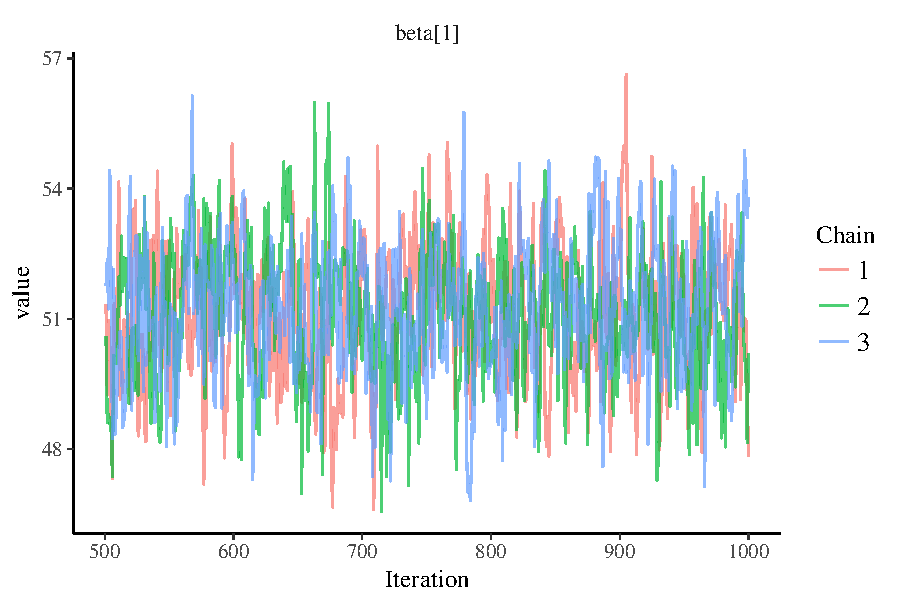
\includegraphics[scale =.3]{gfx/traceplot.pdf}
							\caption{Real}	
							\vspace{.25cm}
						\end{subfigure}
			\\
						\begin{subfigure}[b]{1\textwidth}
							\centering
							\only<3>{										
							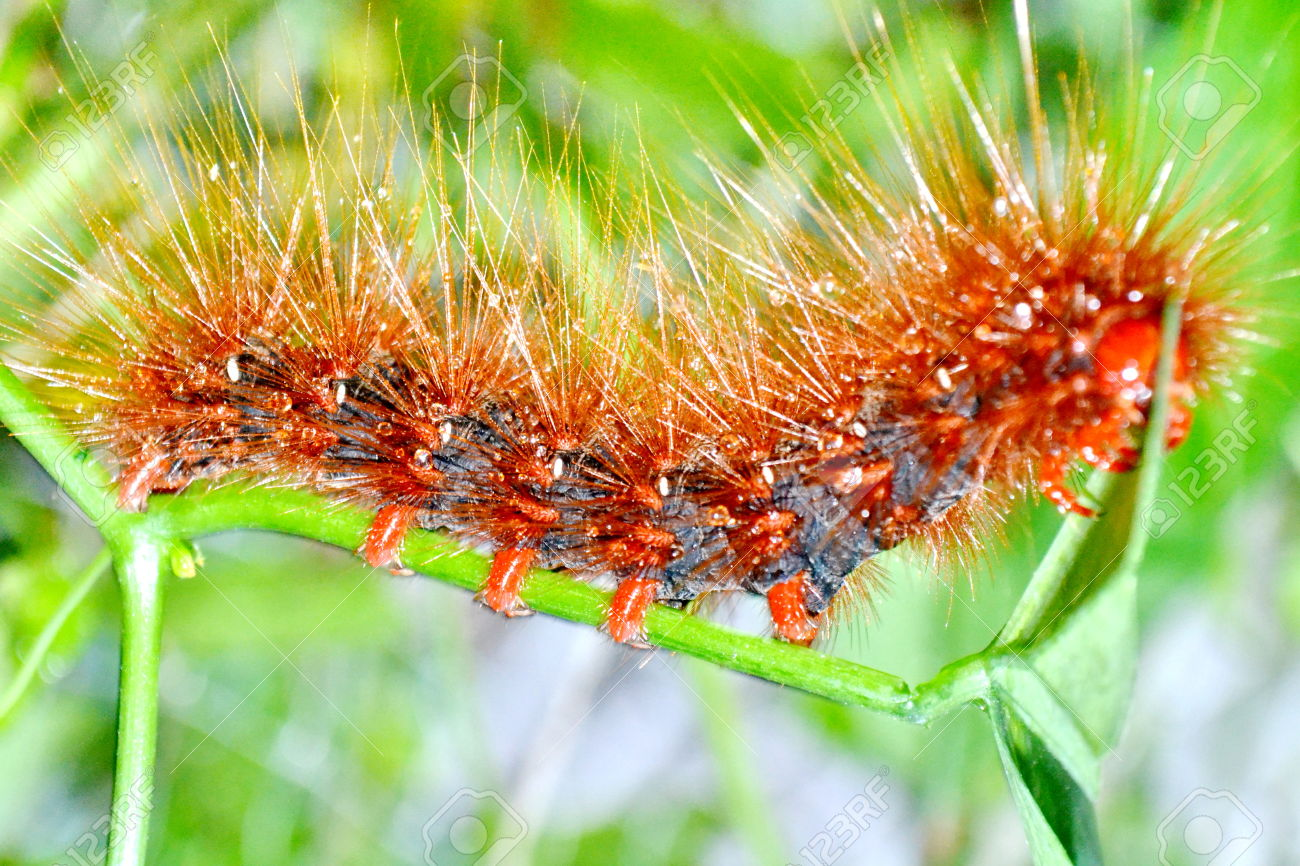
\includegraphics[scale =.3]{gfx/caterpillar.jpg}
							\caption{Fake}	
						}
						\end{subfigure}
			\caption{Traceplots}
		\end{figure}
	}
		\end{minipage}
		

\end{frame}

\begin{frame}
	\frametitle{Bayesian linear mixed effects models}
	
		\begin{figure}
			\centering
			\begin{subfigure}[b]{.45\textwidth}
				\centering
				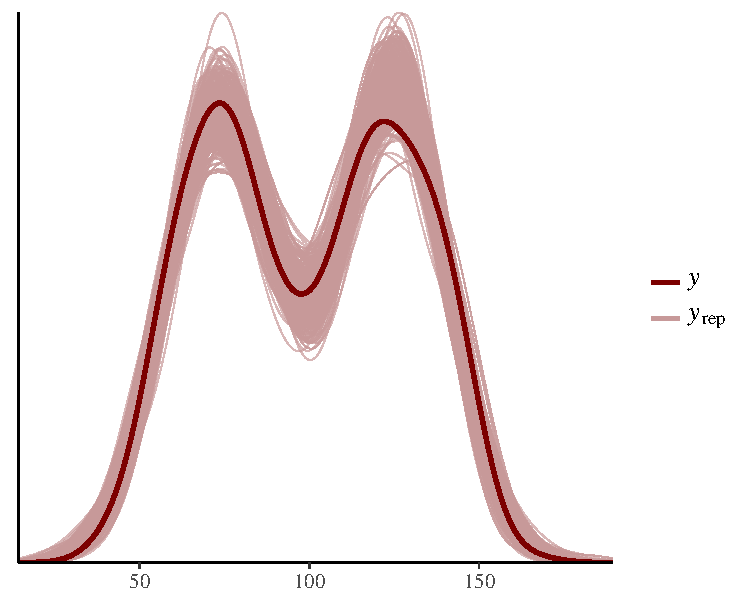
\includegraphics[scale =.4]{gfx/overlay.pdf}
				\caption{Distribution}	
			\end{subfigure}
			\hfill
			\begin{subfigure}[b]{.45\textwidth}
				\centering
				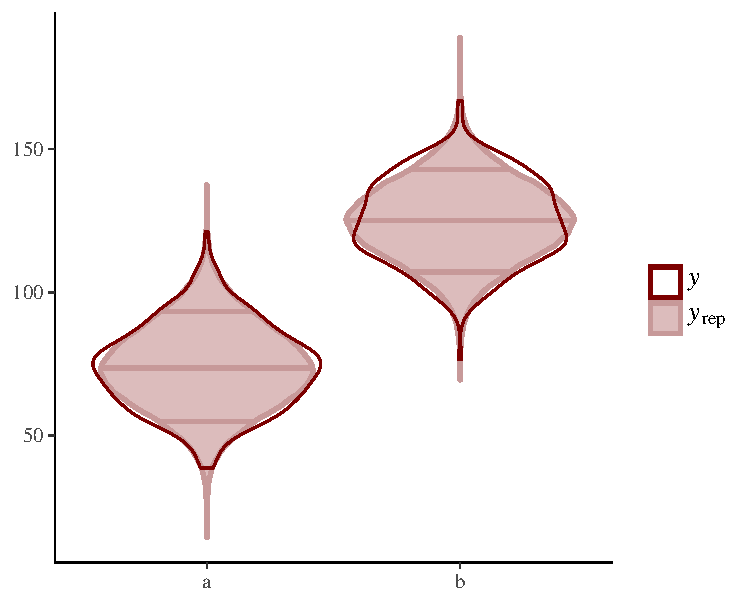
\includegraphics[scale =.4]{gfx/overlaycond.pdf}
				\caption{By-cond}	
			\end{subfigure}
			\caption{Comparison of data and posterior predictive values}
		\end{figure}
	
	
\end{frame}






\begin{frame}
	\frametitle{Bayesian linear mixed effects models}
	
	\begin{itemize}
		\item Does the interval contain 0? Is 0 a possible parameter value? 		
		\item 95\% credible interval (CrI): range of possible parameter values with equal probability mass assigned to each tail (percentile intervals)
		\item 95\% highest posterior density interval (HPDI): interval that embraces the assigned probability mass; identical to CrI for symmetrically distributed posteriors
		\item Go through script $BLMM\_CrI.R$
	\end{itemize}
\end{frame}


\begin{frame}
	\frametitle{Bayesian linear mixed effects models}
	
	\begin{itemize}
		\item Does the interval contain 0? Is 0 a possible parameter value? \only<1>{\item What's the probability that this isn't probable?}
		\only<2>{\item What's probability of a slow-down/speed-up?}
		\item $P(\hat{\beta}<0)$: proportion of posterior samples that is smaller than 0 $\rightarrow$ probability that parameter is smaller than 0 (i.e. speed-up)
		\item Go through script $BLMM\_postprob.R$			
	\end{itemize}
\end{frame}

\begin{frame}
	\frametitle{Bayesian linear mixed effects models}
	
	\begin{itemize}
		\item What's the most likely value for unknown parameter?
		\item Maximum A posteriori (MAP): most frequent $\sim$ probable value
		\item Go through script $BLMM\_MAP.R$	
	\end{itemize}
\end{frame}


\begin{frame}
	\frametitle{Bayesian linear mixed effects models}
	\begin{itemize}
		\item Comparing hypotheses (i.e.~models) using Bayes Factors (BF)
		\item $BF_{10}$: support for $H_1$ over $H_0$  
		\item $BF_{10}$ = 2: $H_1$ is two times more likely than $H_0$; convincing?
		\item $BF_{10}$ = 3--5: weak to moderate evidence
		\item $BF_{10}$ $>$ 10: strong support
		\item $BF_{10}$ $<$ .3: evidence against $H_1$
		\item For evidence in favour of $H_0$: $BF_{01}$
		\item Savage-Dickey density ratio \cite{dickey1970weighted}		
		\item see e.g.~\citeA{bag12}, \citeA{dienes2014using},  \citeA{lee2014bayesian}, \citeA{wagenmakers2010bayesian}
		\item Go through script $BLMM\_BF.R$				 
	\end{itemize}
	
\end{frame}


%dividing the height of the posterior for a certain parameter by the height of the prior of the same parameter, at the point of interest. Critically, we can use the height of an approximation of the posterior distribution.




\begin{frame}
	\frametitle{Bayesian linear mixed effects models}
	\begin{itemize}
		\item All you need!		
		\item Model summary: $BLMM\_modelsummary.R$
	\end{itemize}
\end{frame}



\begin{frame}
	\frametitle{Bayesian linear mixed effects models}
	
%	\begin{minipage}{.45\textwidth}
\only<1>{
	\begin{figure}
		\centering
			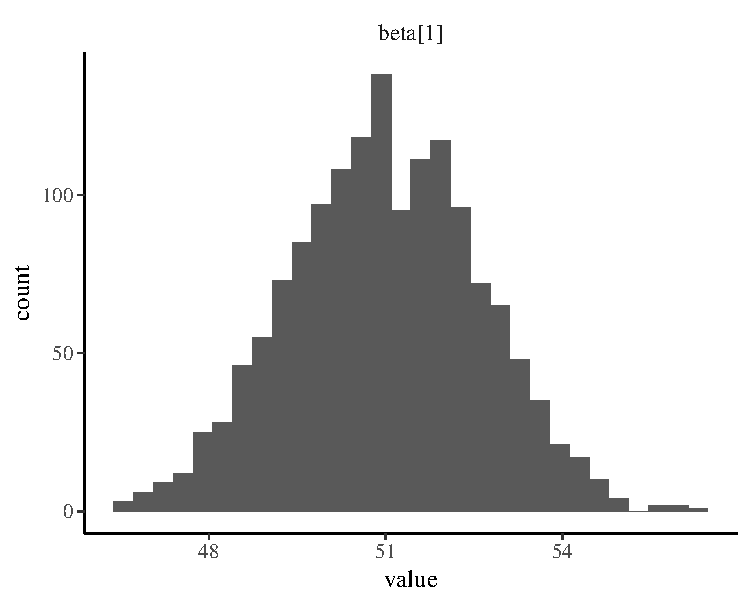
\includegraphics[scale =.65]{gfx/effectdist.pdf}
		\caption{Posterior probability distribution of effect $\hat{\beta}$}
	\end{figure}
}
%	\end{minipage}
%	\hfill
%	\begin{minipage}{.5\textwidth}
\only<2>{
	\begin{table}[!htbp] \centering 
		\caption{Estimates of BLMM. Evidence strongly supports $H_1$ ($BF_{10}>5\times10^{34}$) }
		\begin{tabular}{@{\extracolsep{5pt}} ccccc} 
			\\[-1.8ex]\hline 
			 $\hat{\beta}$ & 2.5\% & 97.5\% & P($\hat{\beta}<0$)   \\ 
			\hline \\[-1.8ex] 
			 51.12 & 47.98 & 54.26 &  $< 0.001$  \\
			\hline \\[-1.8ex] 
			\end{tabular}
		\end{table}
%	\end{minipage}
}
\end{frame}




\begin{frame}
	\frametitle{Bayesian linear mixed effects models}
	
	\begin{itemize}
		\item The future is Bayes!
		\item Existing probabilistic sampling software (Jags, Stan, WinBugs, pyMCMC) makes approximation of posterior easily possible.
		\item Open source access via $R$ and $Python$.
		\item Complex models will converge (easy model fit).
		\item Answers the questions we ask
		\item \dots including support in favour of the null!
		\item No dichotomisation of the significance of the evidence.
		\item Probability distributions of possible parameter values.	
		\item Interpretation of evidence is intuitive.
		\item Custom made models: mixture models, ex-Gaussian 
	\end{itemize}
\end{frame}



\begin{frame}
	\frametitle{Bayesian linear mixed effects models}
	
	\begin{itemize}
		\item Introductions to using Bayesian linear mixed models:
		\begin{itemize}
			\item \citeA{nicenboim2016statistical}: applying $rstanarm$ to psycholinguistic data
			\item \citeA{sorensen2016bayesian}: building LMMs in Stan
		\end{itemize}	
		
		\item Bayesian theory: 
		\begin{itemize}
			\item Great books; with $R$ code: \citeA{kruschke2014doing}, \citeA{mcelreath2016statistical}
			\item Very technical; focus on hierarchical models:  \citeA{gelman2014} 
		\end{itemize}
		
	\end{itemize}
	
\end{frame}